\chapter{相关知识介绍}
\label{ch2}
我们在本章节中介绍了本文研究所需要的一些基本知识,有助于更好的理解之后章节的内容。


\section{联邦学习}
传统的集中式深度学习需要将训练数据放在一起,交给一个数据中心。模型是以集中的方式进行训练的。而联合学习允许数据所有者持有一个私人学习网络,用本地数据集进行训练。之后,每个参与者将本地模型的梯度上传到云服务器。通过更新云服务器上收集的全局梯度,可以避免本地模型的过度拟合。此外,它还可以保护本地数据不被其他参与者或云服务器直接知道。
\subsection{基本定义}



\subsection{联邦学习的分类}
联合学习通常非为水平联邦学习、纵向联邦学习和联合迁移学习,这是由Yang Q等人提出的[8] 。这种分类是基于用户维度和特征维度的重合。
\begin{itemize}
\item \textbf{水平联邦学习}:当两个数据集的用户属性重叠较多而用户重叠较少的情况下,我们对数据集进行横向切割(即按用户维度切割),删除两边用户属性相同但用户不完全相同的那部分数据,用于训练。这种方法被称为横向联合学习。例如,两家银行位于不同的地区,有来自各自地区的用户群,而且它们之间的联系非常少。然而,他们的业务活动非常相似,因此他们的用户特征也是一样的。在这个阶段,我们可以使用跨部门的联合学习来建立一个联合模型。2016年,谷歌提出了一个在安卓手机上更新模型的联合数据建模系统:模型参数在本地不断更新,并在各个用户使用安卓手机时上传到安卓云端,使拥有数据的每一方都能建立一个具有相同特征维度的联合模型。

\item \textbf{纵向联邦学习}:在两个数据集与用户重叠较多而与用户属性重叠较少的情况下,我们将数据集纵向切开(即按特征维度),选择数据集中两边用户相同但用户属性不完全相同的部分进行训练。这种方法被称为纵向的联合学习。例如,有两个不同的组织,一个是在一个地方的银行,另一个是在同一个地方的电子商务公司。他们的用户群很可能包括该地的大部分人口,所以有很大的用户交集。然而,由于银行储存的是用户的收入和支出以及信用评分的数据,而电子商务公司储存的是用户的浏览和购买历史的数据,他们的用户档案并没有那么紧密的联系。长期的联合学习是在一个加密的空间里将这些不同的功能结合起来,以提高模型的性能。渐渐地,人们发现可以在这个联合系统之上建立若干机器学习模型,如逻辑回归、树状结构和神经网络模型。

\item \textbf{联合迁移学习}:联合迁移学习是通过使用迁移学习景观来弥补数据或标签的差距,而不是对数据进行切分,两个数据集中的用户和用户属性几乎没有重叠。这种方法被称为混合式学习迁移。作为一个例子,考虑两个不同的组织,一个是中国的银行,另一个是美国的电子商务公司。由于地理上的限制,这两个机构的用户群重叠的地方很少。由于它们是不同类型的组织,数据的特点也没有太多的重叠。在这种情况下,为了保证有效的联邦学习,有必要引入反式学习,以克服单变量数据量小和标注样本小的问题,提高模型的效率。

\end{itemize}

\subsection{联邦学习的训练步骤}
在很多横向联邦学习应用场景中,参与训练的参与方数据具有类似的数据结构 (特征空间),但是每个参与方拥有的用户是不相同的。有时参与方比较少,例如, 银行系统在不同地区的两个分行需要实现联邦学习的联合模型训练;有时参与方会非常多,例如,做一个基于手机模型的智能系统,每一个手机的拥有者将会是一个独立的参与方。针对这类联合建模需求,可以 通过一种基于服务器客户端的架构来满足很多横向联邦学习的需求。将每一个参与方看作一个客户端,然后引入一个大家信任的服务器来帮助完成联邦学习的联合建模需求。在联合训练的过程中,被训练的数据将会被保存在每一个客户端本地,同时,所有的客户端可以一起参与训练一个共享的全局模型,最终所有的客户端可以一起享用联合训练完成的全局模型。

\begin{itemize}
\item 步骤1:中心服务器初始化联合训练 模型,并且将初始参数传递给每一个客户端。
\item 步骤2:客户端用本地数据和收到的初始化模型参数进行模型训练。具体步骤包括:计算训练梯度,使用加密、差分隐私等加密技术掩饰所选梯度,并将加密后的结 果发送到服务器。
\item 步骤3:服务器执行安全聚合。服务器 只收到加密的模型参数,不会了解任何客 户端的数据信息,实现隐私保护。服务器 将安全 聚合后的结果发送给客户端。
\item 步骤4:参与方用解密的梯度信息更新各自的本地模型,具体方法重复步骤2。
\end{itemize}

\subsection{联邦学习中的安全和隐私威胁}
尽管联邦学习提供了隐私保护的机制,还是有各种类型的攻击方式可以攻击联邦学习系统,从而破坏联邦学习系统安全和参与方的隐私。本节将讨论关于联邦学习的攻击问题。从参与方的类型来看,可 以将联邦学习的威胁模型细分为半诚实模型 (semi-honest model)和恶意模型。对于联邦学习系统的攻击,本文按照不同的维度进行不同层次的分类。从攻击方向角度来看,可以将联邦学习的攻击分为从内部发起和从外部发起两个方面。从攻击者的角色角度来看,可以将攻击分为参与方发起的攻击、中心服务器发起的攻击和第三方发起的攻击。从发动攻击的方式角度来看,可以将攻击分为 中毒攻击和拜占庭攻击。从攻击发起的阶段角度,可以将攻击分为模型训练过程的攻击和模型推断过程的攻击。在密码学领域,基于模型安全的假设通常可以被分为半诚实但好奇(onest but curious)的攻击方假设以及恶意攻击方假设。123123123123

\begin{itemize}

\item \textbf{半诚实但好奇的攻击方}:半诚实但好奇的攻击方假设也被称为 被动攻击方假设。被动攻击方会在遵守联邦学习的密码安全协议的基础上,试图从协议执行过程中产生的中间结果推断或者提取出其他参与方的隐私数据。半诚实但好奇的供给方通常是客户端的角色,它们可以检测从服务器 接收的所有消息,但是不能私自修改训练的 过程。在一些情况下,安全包围或者可信执行环境(trusted execution environment, TEE)等安全计算技术的引入,可以在一定程度上限制此类攻击者的影响或者信息的可见性。半诚实但好奇的参与方将很难从服务器传输回来的参数中推断出其他参与方的隐私信息,从而威胁程度被削弱。

\item \textbf{恶意攻击方}:恶意攻击方也被称为主动攻击方。由于恶意攻击方不会遵守任何协议,为了达到获取隐私数据的目的,可以采取任何攻击手段,例如破坏协议的公平性、阻止协议 的正常执行、拒绝参与协议、不按照协议恶意替换自己的输入、提前终止协议等方式,这些都会严重影响整个联邦学习协议的设计以及训练的完成情况。
恶意的参与方可以是客户端,也可以是服务器,还可以是恶意的分析师或者恶意的模型工程师。恶意客户端可以获取联邦建模过程中所有参与方通信传输的模型 参数,并且进行任意修改攻击。恶意服务器可以检测每次从客户端发送过来的更新模型参数,不按照协议,随意修改训练过程,从而发动攻击。恶意的分析师或者恶意的模型工程师可以访问联邦学习系统的输入和输出,并且进行各种恶意攻击。

\item \textbf{成员推理攻击}:如上文所述,联邦学习机制要求所有参与者通过在本地数据集上训练全局模型来更新梯度。在这种情况下,如果联邦学习系统有一个不被信任的服务器,其知识不能被信任,那么用户的私人信息就不能得到保证。这个不受信任的服务器可以获得关于每个参与者的本地训练模型的大量额外信息(例如,模型结构、用户身份和梯度),并且能够充分损害用户的隐私信息。具体实现如下:攻击者首先在平均化后获得模型的全局参数,并在本地存储这些快照。然后,通过计算以下快照与进一步删除添加的更新,以获得其他用户的模型的汇总更新。通过这种方式,攻击者可以利用数据集的协助,得出所有其他参与者共同合作的数据样本。

\item \textbf{GAN攻击}:Hitaj等人[21]发现,一个联邦学习框架非常容易受到系统内参与者发起的主动攻击。他们首先提出了一个由系统内的恶意用户发起的基于GAN的重建攻击。在训练阶段,攻击者可以冒充无害的用户,训练GAN来模拟由其他用户的训练数据产生的原型样本。通过不断添加假的训练样本,攻击可以逐渐影响整个学习过程,使受害者暴露出更多关于攻击者的目标类的敏感信息。除了客户端发起的GAN攻击,服务器也能通过GAN攻击。恶意服务器最初假装是一个为用户提供联邦学习服务的正常服务器,但其主要目标是重建被攻击用户的训练样本。

\end{itemize}


\section{差分隐私}
差异化隐私作为一种隐私保护方法是为一个用户服务的,因为根据隐私的定义,隐私泄露只是与特定用户有关的信息泄露,而一组用户的统计特征不包括在隐私信息中。如果一个对象在数据库中的存在或不存在,或其价值的变化不会对搜索结果产生重大影响,那么该对象的隐私信息就会受到保护,这就是差异性隐私(DP)概念的起源。差异隐私首先被应用于数据查询,为了更好地说明数据集之间的差异,定义了相邻数据集的概念:两个数据集只差一个信息或只差一个数值不同的记录。因此,查询数据库相关信息的攻击者将无法以任何概率确定$X_{n}$是否存在于数据集中,而成员$X_{n}$被认为是相对安全的。


\subsection{基本定义}
对于一个有限域 $Z, z \in Z$ 为 $Z$ 中的元素, 从 $Z$ 中抽样所得 $z$ 的集合组成数据集 $D$, 其样本量为 $n$, 属性的个数为维度 $d$。对数据集 $D$ 的各种映射函数被定义为查询 (Query), 用 $F=\left\{f_{1}, f_{2}, \cdots\right\}$ 来表示一组查询,算法 $M$ 对查询 $F$ 的结果进行处理,使之满足隐私保护的 条件,此过程称为隐私保护机制。设数据集 $D$ 和 $D^{\prime}$,具有相同的属性结构,两者 的对称差记作 $D \Delta D^{\prime},\left|D \Delta D^{\prime}\right|$ 表示 $D \Delta D^{\prime}$ 中记录的 数量。若 $\left|D \Delta D^{\prime}\right|=1$, 则称 $D$ 和 $D^{\prime}$ 为邻近数据集 (Adjacent Dataset)。
\begin{figure}[!hbt]
\centering
	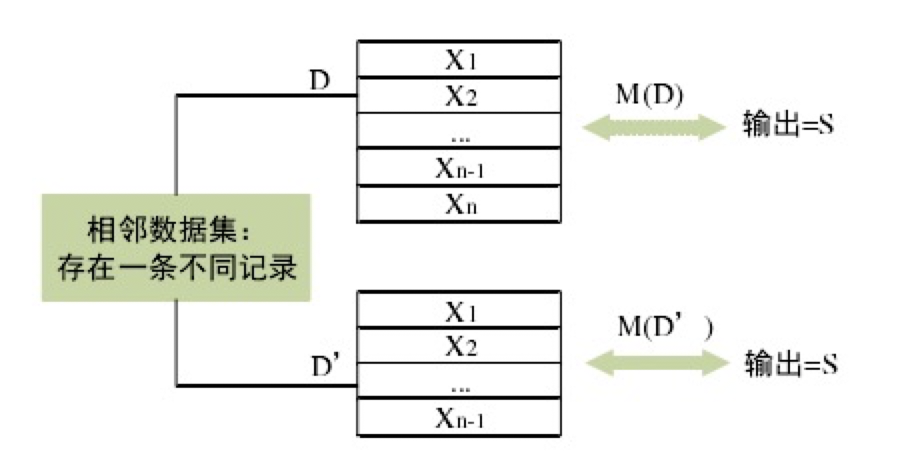
\includegraphics[scale=0.7]{fig2/C2/相邻数据集示意图}%联邦学习的系统架构
	\label{fig:相邻数据集示意图}	
\end{figure}


\begin{define}[成立条件]\label{成立条件}

若随机算法 $M: D \rightarrow R$ 满足 $(\varepsilon, \delta)-D P$, 当且仅当相邻数据集 $d, d^{\prime}$ 对于算法 $M$ 的所有可能输出子集 $S \in R$ 满足不等式 $^{[40]}$ :
$$
\operatorname{Pr}[M(d) \in S] \leq e^{\varepsilon} \operatorname{Pr}\left[M\left(d^{\prime}\right) \in S\right]+\delta
$$

其中,$\varepsilon$ 表示隐私预算参数, $\varepsilon$ 越小意味着隐私预算越低, 信息泄露越少,隐私保护的强度越高。添加项 $\delta$代表允许以概率 $\delta$ 打破 $\varepsilon-\mathrm{DP}$ 的可能性, 其值通常选择为小于 $1 /|D|$. 当 $\delta=0$ 时, 定义转化为 $\varepsilon-\mathrm{DP}$, 这时机制提供了更加严格的隐私保护。隐私预算参数决定着隐私保护强度, 针对传统数据库保护,当 $\varepsilon \in(0,1)$ 时认为隐私保护强度是有效的, 但 应用在深度学习领域, $\varepsilon \in(0,10)$ 都认为是可以被接受的合理范围。
如图 1 所示,算法 $M$ 通过对输出结果的随机化 来提供隐私保护,同时通过参数 $\varepsilon$ 来保证在数据集中删除任一记录时,算法输出同一结果的概率不发生显著变化。
\end{define}

\subsection{相关概念}
差分隐私保护可以通过在查询函数的返回值中 加人适量的干扰噪声来实现. 加人噪声过多会影响 结果的可用性,过少则无法提供足够的安全保障. 敏感度是决定加人噪声量大小的关键参数, 它指删除 数据集中任一记录对查询结果造成的最大改变. 在差分隐私保护方法中定义了两种敏感度, 即全局敏感度(Global Sensitivity)和局部敏感度(Local Sensitivity).

\begin{define}[全局敏感度]\label{全局敏感度}
设有函数 $f: D \rightarrow R^{d}$, 输人为一数据集,输出为一$d$ 维实数向量. 对于任意的邻近数据集 $D$ 和 $D^{\prime}$,
$$
G S_{f}=\max _{D, D^{\prime}}\left\|f(D)-f\left(D^{\prime}\right)\right\|_{1}
$$
称为函数 $f$ 的全局敏感度。
函数的全局敏感度由函数本身决定,不同的函数会有不同的全局敏感度.一些函数具有较小的全局敏感度(例如计数函数,其全局敏感度为1),因此只需加入少量噪声即可掩盖因一个记录被删除对查询结果所产生的影响,实现差分隐私保护。
\end{define}

\begin{define}[局部敏感度]\label{局部敏感度}
对于一个查询函数 $f_{:} D \rightarrow R^{d}$, 其中 $D$ 为一个数据集, $R^{d}$为d维实数向量,是查询的返回结果。对于给定的数据集D和它的任意邻近数据集 $D^{\prime}$, 有 $f_{\text {在 }} D$ 上的局部敏感度为:
$L S_{f}(D)=\max _{D^{\prime}}\left\|f(D)-f\left(D^{\prime}\right)\right\|_{1}$

局部敏感度由函数犳及给定数据集犇中的具体数据共同决定.由于利用了数据集的数据分布特征, 局部敏感度通常要比全局敏感度小得多。
敏感度代表了查询函数针对相邻数据集的输出的最大不同,或者说量化评估了最坏情况下单个样本对整体数据带来的不确定性大小。敏感度函数仅与查询函数的类型有关, 为扰动的添加提供了依据。但是,由于局部敏感度在一定程度上体现了数据集的数据分布特征,如果直接应用局部敏感度来计算噪声量则会泄露数据集中的敏感信息。
\end{define}

全局差分隐私技术旨在实现这样一个目标:如果替换数据集中的任意样本的效果足够小,则查询结果不能被用来探索数据集中任何样本的更多信息[43]。作为一种优势,这种技术比局部差分隐私技术更准确,因为它不需要向数据集添加大量的噪声。局部差分隐私技术被引入以去除全局差分隐私中所要求的受信任的中央机构[34,102]。与全局差分隐私技术相比,局部差分隐私技术不需要可信的第三方[146]。其缺点是,噪声总量比全局差分隐私技术大得多。


在差分隐私部署过程中常常不仅仅在一处添加噪声, 也不仅仅针对数据集进隐私预算的分配有序列组合性[41]和并行组合性 ${ }^{[42]}$ 两种组合特性:

\begin{define}[序列组合]\label{序列组合}
给定 $\mathbf{n}$ 个陏机算法 $M_{i}(1 \leq i \leq n)$ 满足 $\varepsilon_{i}-DP$, 那么针对一个数据库 $D$ 而言, 在 $\mathrm{D}$ 上的算法序列组合可以提供 $\varepsilon-\mathrm{DP}$, 其中 $\sum_{i=1}^{n} \varepsilon_{i}=\varepsilon$ 。
\end{define}

\begin{define}[并行组合]\label{并行组合}
对于数据库 $\mathrm{D}$, 当其被划分成 $\mathrm{n}$ 个不相交的子集 $\left\{\mathrm{D}_{1}, \mathrm{D}_{2}, \ldots, \mathrm{D}_{n}\right\}$, 在每个子集上应用算法 $\mathrm{M}_{i}$, 每个算法提供 $\varepsilon_{i}-\mathrm{DP}$ , 则在序列 $\left\{\mathrm{D}_{1}, \mathrm{D}_{2}, \ldots, \mathrm{D}_{n}\right\}$ 上整体满足 $\left(\max \left\{\varepsilon_{1}, \ldots, \varepsilon_{n}\right\}\right)-\mathrm{DP}$
\end{define}


\subsection{实现机制}
在实践中为了使一个算法满足差分隐私保护的要求,对不同的问题有不同的实现方法,这些实现方法称为“机制”.拉普拉斯机制(Lapalace Mechanism)、指数机制[22](ExponentialMechanism)与高斯机制是三种最基础的差分隐私保护实现机制.其中,Laplace机制和高斯适用于对数值型结果的保护,指数机制则适用于非数值型结果。

在中心化差分隐私中,最为常用的扰动机制是拉普拉斯(Laplace)机制,该机制可以后期处理聚合查询(例如,计数、总和和均值)的结果以使它们差分私有。
Laplace分布是统计学中的概念,是一种连续的概率分布。

\begin{define}[拉普拉斯机制]\label{拉普拉斯机制}
如果随机变量的概率密度函数分布为:

$f(x \mid \mu, b)=\frac{1}{2 b} \exp \left(-\frac{|x-\mu|}{b}\right)=\frac{1}{2 b}\left\{\begin{array}{ll}\exp \left(-\frac{\mu-x}{b}\right) & x<\mu \\ \exp \left(-\frac{x-\mu}{b}\right) & x \geq \mu\end{array}\right.$

其中,D表示数据集,$f(D)$表示的是查询函数,$Y$表示的是Laplace随机噪声,$M(D)$表示的是最后的返回结果。
$M(D)=f(D)+Y$
如果噪声 $Y \sim L\left(0, \frac{\Delta f}{\longrightarrow}\right)$ 满足 $(\epsilon, 0)-$,则表示服从拉普拉斯分布的随机噪声。因此,当隐私预算$\mathbf{3}$确定时,敏感度越大,引入的噪声量越大。
\end{define}

对于非数值型的查询结果或数据,通常使用指数机制来随机选择离散的输出结果来满足差分隐私。指数机制整体的思想就是,当接收到一个查询之后,不是确定性的输出一个$R_{i}$结果,而是以一定的概率值返回结果,从而实现差分隐私。而这个概率值则是由打分函数确定,得分高的输出概率高,得分低的输出概率低。

\begin{define}[指数机制]\label{指数机制}
指数机制满足差分隐私, 如果:

$M(D)=\left(\right.$ return $\left.\varphi \propto \exp \left(\frac{\varepsilon q(\mathrm{D}, \varphi)}{2 \Delta q}\right)\right)$

评分函数 $\mathrm{q}(\mathrm{D}, \varphi)$,用于评估输出 $\varphi$ 的质量。$\Delta q$ 代表了输出的敏感度。
\end{define}


\section{神经网络}
如图\ref{fig:深度神经网络结构图}所示,深度神经网络基于模块化思想,通过在多个层次上部署多个神经元并通过逐层训练的手段调整神经元间的连接权值,从而实现原始特征数据进行多次非线性变换,对于任何有限给定输入/输出数据的拟合,最终获取到稳定的特征用于后续的问题分析。
\begin{figure}[!hbt]
\centering
	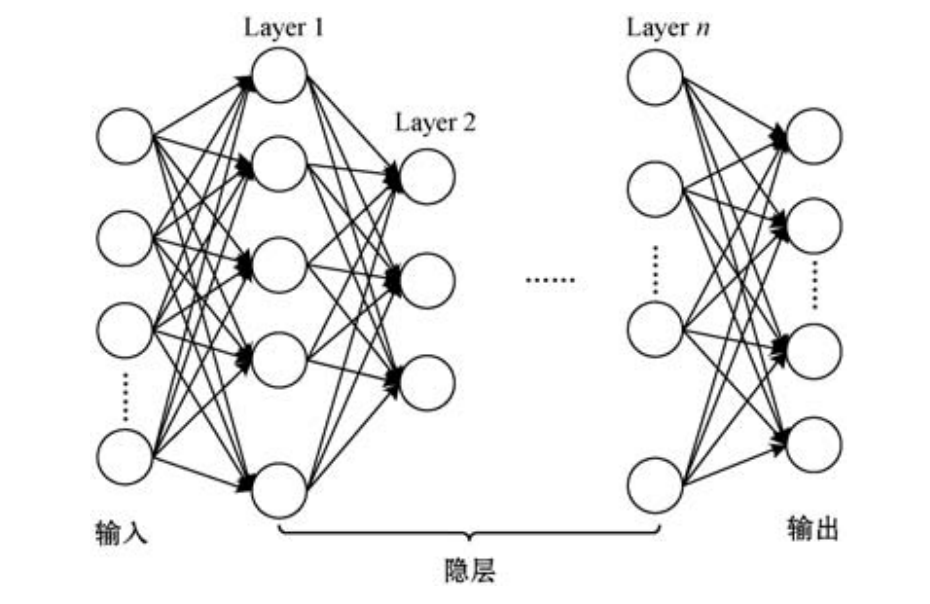
\includegraphics[scale=0.7]{fig2/C2/深度神经网络结构图}%联邦学习的系统架构
	\label{fig:深度神经网络结构图}	
\end{figure}

深度神经网络算法中,为评估所提神经网络输出预测值与真实值之间的差异程度,用损失函数 $L$ 表示, 文中采用均方差损失函数,表示为:
$$
L(\theta, x)=\frac{1}{n} \sum_{i=1}^{n}\left(y_{i}-x_{i}\right)^{2}
$$
式中: $\theta$ 为待训练的神经网络权重系数; $x$ 表示目标值; $y$ 表示预测值输出,下标 $i$ 表示样本标签。深度神经网 络算法训练的目的就是使得损失函数 $L$ 最小。而对于 复杂的神经网络而言,最小化损失函数 $L$ 通常采用随机 梯度下降( stochastic gradient descent, SGD)算法来完成。 即每次迭代过程中随机进行批量抽取训练样本 (记为 $B)$, 并计算损失函数 $L$ 的偏导数 $g_{B}=\frac{1}{|B|} \sum_{x \in B} \nabla_{\theta} L(\theta,$, $x$ ),然后沿着负梯度方向 $-g_{B}$ 朝向局部最小值进行更 新权重系数 $\theta_{\circ}$

\section{本章小结}


